\subsection{Analyse}

\subsubsection{Statisk analyse}
\begin{figure}[htb!]
  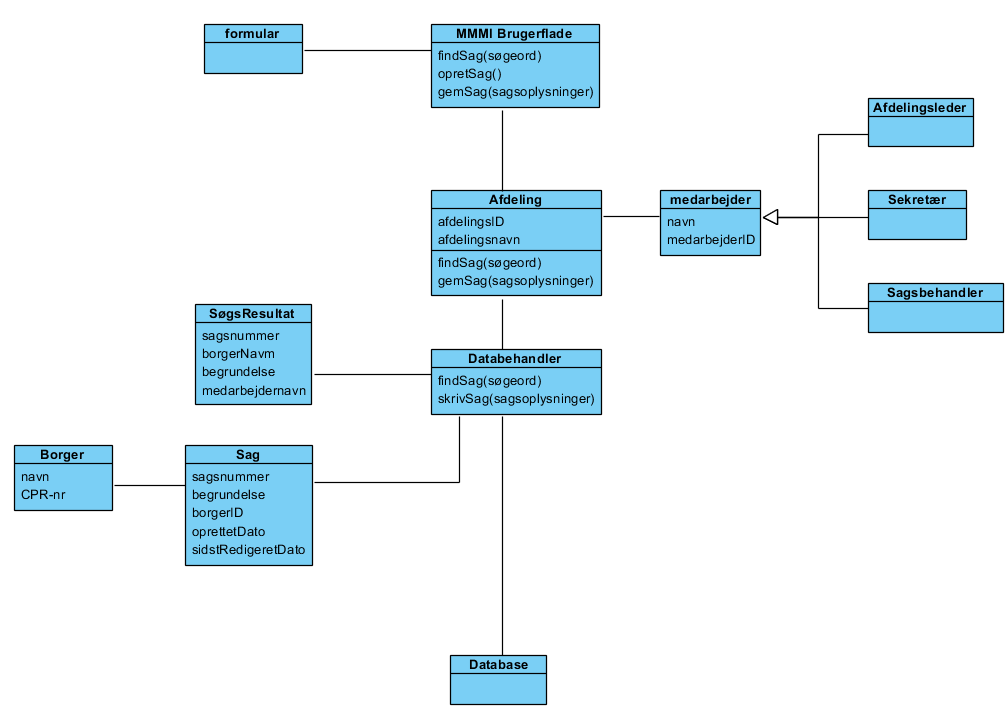
\includegraphics[scale = 0.7]{./PNG/analyse/analyseklassediagramOpdateret.PNG} 
  \caption{Analyse klasse diagram opdateret til anden iteration}
  \label{fig:2analyseklasse}
\end{figure}
Da der har været fokus på at få integreret en database og en funktionel grafisk brugergrænseflade i 2. iteration, består de primære ændringer i den statiske analyse, af arbejdet med at revidere klassediagrammet, med henblik på at tilføje persistens og præsentation. Der er bl.a. blevet ændret på hvordan de tre klasser der repræsenterer ansatte, og klassen der repræsenterer borgere, beskrives. \\
Der blev valgt at gå væk fra en overordnet abstrakt klasse (Se figur \ref{fig:AKlasse})kaldet ”Person”, som ”Borger”, ”Afdelingsleder”, ”Sekretær” og ”Sagsbehandler” klasserne arvede fra. En abstrakt klasse kaldet ”medarbejder” blev lavet, som ”Afdelingsleder”, ”Sekretær” og ”Sagsbehandler” arvede fra i stedet, og holdt ”Borger” som en separat klasse. Dette betød at ”Borger” fik navn og CPR-nr. som attributter, til forskel fra 1. iteration hvor den kun havde CPR-nr. og arvede navn fra ”Person”. Yderligere blev medarbejderID flyttet til superklassen, da alle arvende klasser skulle bruge den. \\
Det blev droppet at beholde ”Afgørelsesbrev” som klasse, da det gav mere mening at lægge den i præsentationslagets klasse ”Formular”, som også repræsenterer alle andre formularer der beskrives i VUM.\\
Klassen ”Sag” er blevet rykket ned til datalaget og kan tilgås gennem Databehandler klassen, som er den klasse der repræsenterer datalaget og skal varetage al kommunikation med databasen.\\
De vigtigste metoder og attributter, på diverse klasser, er blevet opdateret i forhold til den nye viden, der er blevet indsamlet gennem 2. iteration. Der er blevet lavet nye metoder er på klassen (Se figur \ref{fig:2analyseklasse})”MMMI Brugerflade”, som er ”findSag”, ”opretSag” og ”gemSag”. På klassen ”Afdeling” er metoderne ”findSag” og ”gemSag” blevet lavet og på klassen ”Databehandler” er ”findSag” og ”skrivSag” blevet lavet. De nye attributter som er tilføjet, er ”begrundelse”, ”borgerID”, ”oprettetDato” og ”sidstRedigeretDato” på ”Sag”. \\
Den nye klasse ”SøgsResultat”, bruges til at holde data samlet i forbindelse med en given søgning af en sag. De attributter som vises i klassen ”SøgsResultat”, repræsenterer en begrænset delmængde af hvad der gemmes når en sag oprettes, men det er nok til at en bruger vil være i stand til at identificere en given sag for at åbne den.\\
Klassen Database repræsenterer den postgresql database er blevet implementeret i iteration 2.

\subsubsection{Dynamisk analyse}
I anden iteration er der blevet udarbejdet operationssekvensdiagrammer i forhold til ”opretSag()”, ”opdaterSag()” og ”find()”. \\
Operationen ”opretSag()” (Se afsnit \underline{\ref{opret} opretSag}) og ”opdaterSag()” (Se afsnit \underline{\ref{opdaterSag} opdaterSag}) er operationer der stammer fra opretSag fra første iteration. I de pågældende sektioner vil der beskrives de overvejelser der blevet fortaget i forhold til de to operationer samt beskrivelse og vurdering. \\
Operationen find() er den operation der stammer fra ”findSag()” fra første iteration. I afsnit \underline{\ref{find} find} beskrives der overvejelserne om f.eks. fra ”findSag()” til find() og beskrivelse samt vurdering af operationen.\\ 
\textbf{opretSag():} \label{opret} \\ 
Operationen ”opretSag()” er den funktion der opretter en sag i systemet. Der gjort overvejelser om at håndtere opdaterSag() i samme funktion som ”opretSag()”, men det ville ikke give mening samtidig med at det ville gøre diagrammet uoverskueligt. Derfor er de adskilt i to operationer. \\
\begin{figure}[htb!]
  \includegraphics[scale = 0.5]{./PNG/analyse/opretsag2.PNG} 
  \caption{Sekvensdiagram for opret sag opdateret til anden iteration Se interne bilag \ref{sec:diverse} figur \ref{fig:2fopretsag}}
  \label{fig:2opret}
\end{figure}
I figur \ref{fig:2opret}. begynder funktionen ved at en sagsbehandler eller sekretær vælger ”opretSag()”. Brugergrænsefladen returner en sagsåbningsformular, som skal udfyldes. Når sagsbehandleren har indtastet sagsoplysningerne vælger sagsbehandler at gemme sagen. Operationen ”gemSag()” sender besked til Afdeling som derefter benytter operationen ”skrivSag()” til Databehandleren og til sidst sender Databehandleren beskeden videre til databasen. Databasen returner en bekræftelse tilbage til Databehandleren som returner den igennem Afdeling og til sidst fortæller aktøren at sagen blev oprettet. \\
Ved at anvende ”opretSag()” operationen har en sagsbehandler eller sekretær mulighed for at vælge en formular og udefra den gemme den og dermed oprette en ny sag. Oprettelsen sker når borgeren henvender sig og dermed kan sekretæren eller sagsbehandleren oprette en sag på den pågældende borger. For at kunne håndtere om en borger allerede har en sag eller om der findes oplysninger om borgen, benyttes ”find()” operation, som kan læses i afsnit \underline{\ref{find} find}\\
\textbf{opdaterSag():} \label{opdaterSag}\\
Operationen ”opdaterSag()” med en kombination af ”find()” operationen gør det muligt for en aktør at kunne finde en specifik sag og dermed åbne den og opdatere den. \\
\begin{figure}[htb!]
  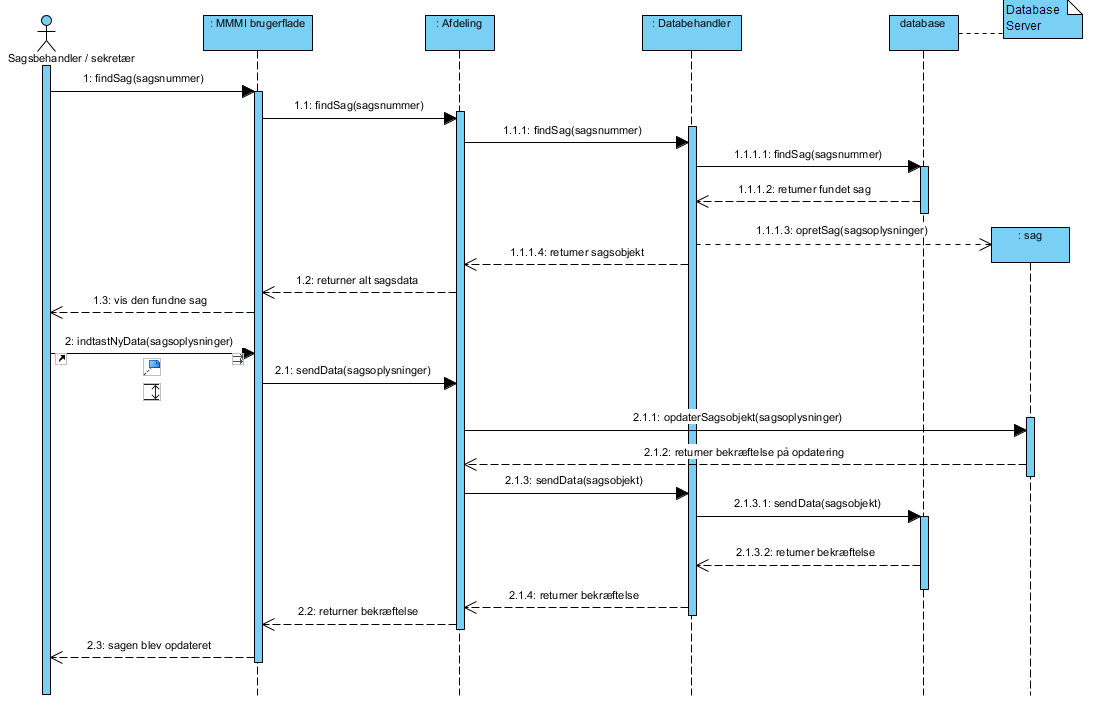
\includegraphics[scale = 0.62]{./PNG/analyse/opdaterSag.PNG} 
  \caption{Sekvensdiagram for opdater sag opdateret til anden iteration}
  \label{fig:2opdater}
\end{figure}
I figur \ref{fig:2opdater} ses det at en sagsbehandler eller sekretæren vælger at fremsøge en sag. ”findSag()” beskeden bliver sendt igennem afdelingen og databehandleren. Databehandleren sørger for at sende beskeden til databasen og fremskaffe den søgte sag. Denne returneres til databehandleren og der bliver oprettet et sagsobjekt. Dette sagsobjekt returneres til afdelingen og herefter til brugerfladen og til sidst bliver den vist til brugeren. Når brugeren vælger at ”indtastNyData()” til det pågældende sagsobjekt, med de pågældende sagsoplysninger sendes til afdelingen via operationen ”sendData()”. Afdelingen sørger for at opdater sagsobjektet igennem beskeden ”opdaterSagsobjekt()” hvor sag returner sagsobjekt med sagsoplysningerne og det sagsobjekt og data sendes til Databehandleren igennem beskeden ”sendData()” som derefter sender besked til databasen om at gemme de nye oplysninger. Databasen returner en bekræftelse igennem databehandleren, afdelingen og til sidst sendes det til brugerfladen som så bekræfter overfor aktøren at sagen blev opdateret. \\
Det vurderes at denne operation er en væsentlig del af sagsforløbet og skulle kunne muliggøre for en sagsbehandler eller sekretær at kunne opdatere en sag ved at kombinere operationen med at finde en sag først og derefter opdatere den. \\
\textbf{find():} \label{find}\\
\begin{figure}[htb!]
  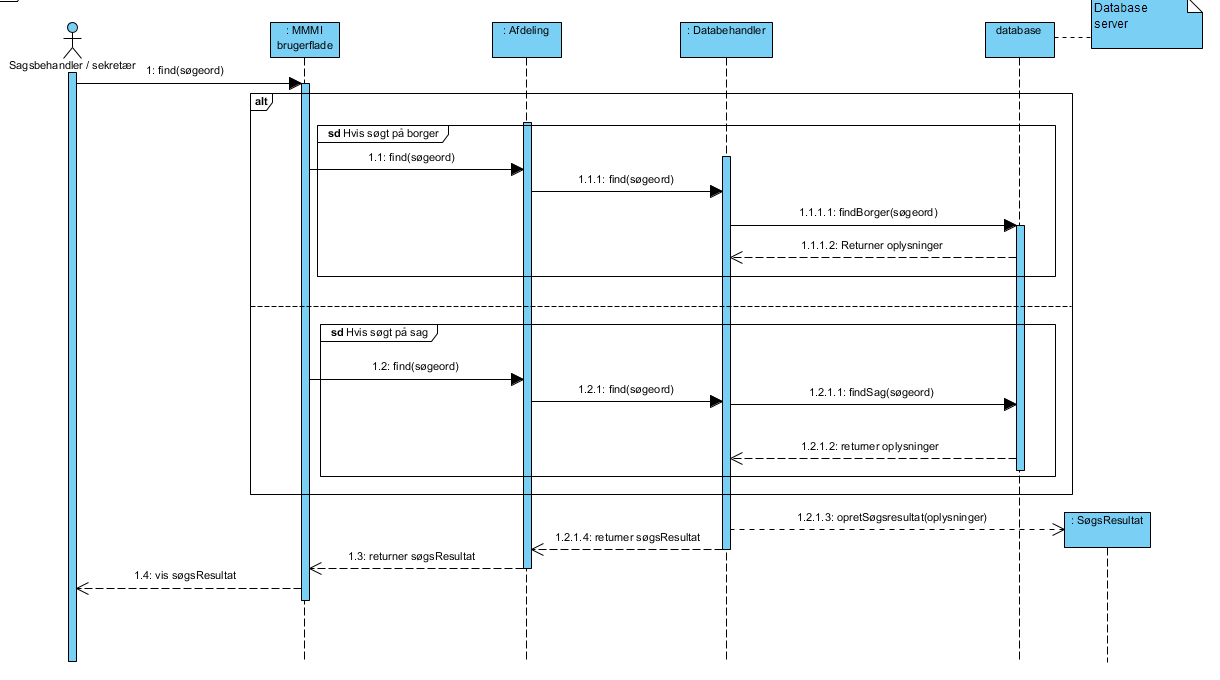
\includegraphics[scale = 0.56]{./PNG/analyse/find.PNG} 
  \caption{Sekvensdiagram for find sag opdateret til anden iteration}
  \label{fig:2find}
\end{figure}
Tanken med ”findSag()” i første iteration afsnit … har været at kunne fremsøge en pågældende sag frem. Der har været overvejelser om at kunne fremsøge en borger og en sag, fra en enkelt operation. Derfor blev ”findSag()” operationen lavet om til en mere general operation kaldt ”find()”.\\
I figur \ref{fig:2find} vælger en sagsbehandler eller sekretær at finde en sag eller borger baseret på et søgeord. Operationen ”find()” sender besked til grænsefladen. Baseret på den pågældende søgning, hvis det er en borger eller en sag der søges på, sendes ”find()” besked videre fra Afdelingen til Databehandleren der sørger for at sende besked til databasen, hvor der efterfølgende sendes svar fra databasen til Databehandleren der så baseret om det er en sag eller borger der er søgt på, opretter et SøgsResultat objekt, som Databehandleren sender tilbage. Afdelingen sørger for at sende beskeden til brugerfladen som til sidst viser søges resultatet til aktøren. \\
At kunne finde en sag frem eller en specifik borger er en vigtig funktion og dermed en vigtig operation for en sagsbehandler eller sekretær. Denne operation hjælper med at kunne finde sag på en pågældende borger og dermed hjælpe mere effektivt, ved at kunne hente alle sagsoplysninger. \\ 
